%%%%%%%%%%%%%%%%%%%%%%%%%%%%%%%%%%%%%%%%%
% Journal Article
% LaTeX Template
% Version 1.3 (9/9/13)
%
% This template has been downloaded from:
% http://www.LaTeXTemplates.com
%
% Original author:
% Frits Wenneker (http://www.howtotex.com)
%
% License:
% CC BY-NC-SA 3.0 (http://creativecommons.org/licenses/by-nc-sa/3.0/)
%
%%%%%%%%%%%%%%%%%%%%%%%%%%%%%%%%%%%%%%%%%

%----------------------------------------------------------------------------------------
%	PACKAGES AND OTHER DOCUMENT CONFIGURATIONS
%----------------------------------------------------------------------------------------

\documentclass[twoside]{article}

\usepackage{lipsum} % Package to generate dummy text throughout this template

\usepackage{amsmath,amsthm,amssymb}

\usepackage[hmarginratio=1:1,top=32mm,columnsep=20pt]{geometry} % Document margins
\usepackage{multicol} % Used for the two-column layout of the document
\usepackage[hang, small,labelfont=bf,up,textfont=it,up]{caption} % Custom captions under/above floats in tables or figures
\usepackage{booktabs} % Horizontal rules in tables
\usepackage{float} % Required for tables and figures in the multi-column environment - they need to be placed in specific locations with the [H] (e.g. \begin{table}[H])
\usepackage{hyperref} % For hyperlinks in the PDF
\usepackage[export]{adjustbox}
%\usepackage{subcaption}

\usepackage{array}
\usepackage{paralist} % Used for the compactitem environment which makes bullet points with less space between them

\usepackage{abstract} % Allows abstract customization
\renewcommand{\abstractnamefont}{\Large\normalfont\bfseries} % Set the "Abstract" text to bold
%\renewcommand{\abstracttextfont}{\normalfont\small\itshape} % Set the abstract itself to small italic text

\usepackage{titlesec} % Allows customization of titles
\titleformat{\section}[block]{\Large\bf\scshape\centering}{\thesection.}{0.25em}{} % Change the look of the section titles
%\titleformat{\subsection}[block]{\large}{\thesubsection.}{1em}{} % Change the look of the section titles

\usepackage{fancyhdr} % Headers and footers
\usepackage{graphicx}
%\usepackage{subfigure}
\usepackage{wrapfig}
\usepackage{subfig}
\usepackage{cancel}
\usepackage[normalem]{ulem}
\usepackage{color}

%\pagestyle{fancy} % All pages have headers and footers
%\fancyhead{} % Blank out the default header
%\fancyfoot{} % Blank out the default footer
%\fancyhead[C]{Running title $\bullet$ November 2012 $\bullet$ Vol. XXI, No. 1} % Custom header text
%\fancyfoot[RO,LE]{\thepage} % Custom footer text

%----------------------------------------------------------------------------------------
%	TITLE SECTION
%----------------------------------------------------------------------------------------

\title{\vspace{-15mm}\fontsize{20pt}{10pt}\selectfont\textbf{Application of Compressive Sensing ideas to Static Electromagnetic Geophysics}} % Article title
\author{
\Large
\textsc{EOSC 513: Course Project}
\\\\
\large
\textsc{Thibaut Astic}\\%Or \normalsize for text
\textsc{90142150} \\ % Your institution
\normalsize thast@eos.ubc.ca
\vspace{-5mm}
}
\date{}

%----------------------------------------------------------------------------------------

\begin{document}

\newcommand*{\vertbar}{\rule[-1ex]{0.5pt}{2.5ex}}
\newcommand*{\horzbar}{\rule[.5ex]{2.5ex}{0.5pt}}

\maketitle % Insert title

%\thispagestyle{fancy} % All pages have headers and footers

%----------------------------------------------------------------------------------------
%	ABSTRACT
%----------------------------------------------------------------------------------------

\begin{abstract}

DC Resistivity (DCR) is a static electromagnetic surveying method. It is primarily used for near-surface characterization of buried infrastructure, mineral deposit, archeology and forensic investigation (\cite{YO:1996}). The diagnostic physical property for DCR is electrical conductivity $\sigma$ (or its inverse resistivity $\rho$), which is mainly influenced by water and metal contents.

A set of strategies have been successfully used in SimPEG (\cite{CKH+:2015}), an open source package for electromagnetic Geophysics, for inverting DCR data using a finite volume discretization. These strategies include the formulation of a L2-regularized objective function, which is then solved by updating a linearized version of the residual term thanks to an inexact Gauss-Newton step. The regularizer's weight is also regularly updated following a cooling strategy.

We propose in this project to apply some of the Compressive Sensing ideas to a DCR inverse problem. 

Our first step will be to reformulate the inverse problem as a stochastic programming problem using simultaneous sources, as it has been applied recently in (\cite{HCH:2012}). We will present the impact of several strategies for the choices of the random matrix in term of its nature, size and updates. 

Our next step will be to promote sparsity in the Gauss-Newton subproblem in a transformed domain. For this purpose we will be using the SPGl1 package presented in (\cite{BF:2008}). This approach will help us to get additional highlights on our data such as for example the depth of investigation by exploring the possible models space in a different way.

Our open-source code has been made publicly available through \href{https://github.com/thast/EOSC513}{Github},  to ensure an easy reproducibility of the results presented in the final report as this has been a growing need in Geophysics and Sciences in general (\cite{SEG:2016}).


\end{abstract}

%----------------------------------------------------------------------------------------
%	ARTICLE CONTENTS
%----------------------------------------------------------------------------------------

%\begin{multicols}{2} % Two-column layout throughout the main article text

\section{Introduction}

Characterizing the Earth's subsurface is one of the key questions in Earth Sciences, either to image the Earth's core, anticipating pollution migration, finding minerals resources etc. Geophysics goal is to image these structures remotely by measuring Earth's response to different fields. 

One of the main group of methods used in Geophysics are the electromagnetic methods (\cite{WH:1988}). With this project we are going to particularly focus on a static Electromagnetic method, DC Resistivity (DCR, figures \ref{DC_setup} and \ref{DC_pot_fields}). Electromagnetic phenomenons are governed by Maxwell's equations and hence are sensitive to contrasts in physical properties that can be interpreted in terms of geologic structure and fluid content. The diagnostic physical property for DCR is electrical conductivity $\sigma$ (or its inverse resistivity $\rho$). In a nutshell, DC Currents are injected into the ground thanks to a generator imposing a potential difference at the sources electrodes (electrodes A and B in figures \ref{DC_setup} and \ref{DC_pot_fields}). The path of the currents are determined by the electrical conductivity contrasts in the subsurface. Data are acquired either at the surface or in boreholes by measuring potential differences between measurements electrodes (electrodes M and N in figures \ref{DC_setup} and \ref{DC_pot_fields}).

\begin{figure}[!ht]
\centering
\begin{minipage}{0.5\textwidth}
  \centering
    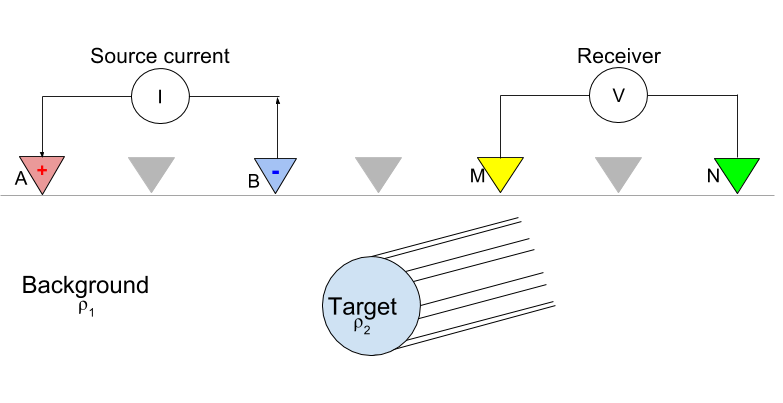
\includegraphics[width=.9\linewidth]{figures/DCR_Setup_Cylinder.png}
  \captionof{figure}{DCR system for a single source over a cylindrical target}
  \label{DC_setup}
\end{minipage}%
\begin{minipage}{.5\textwidth}
  \centering
  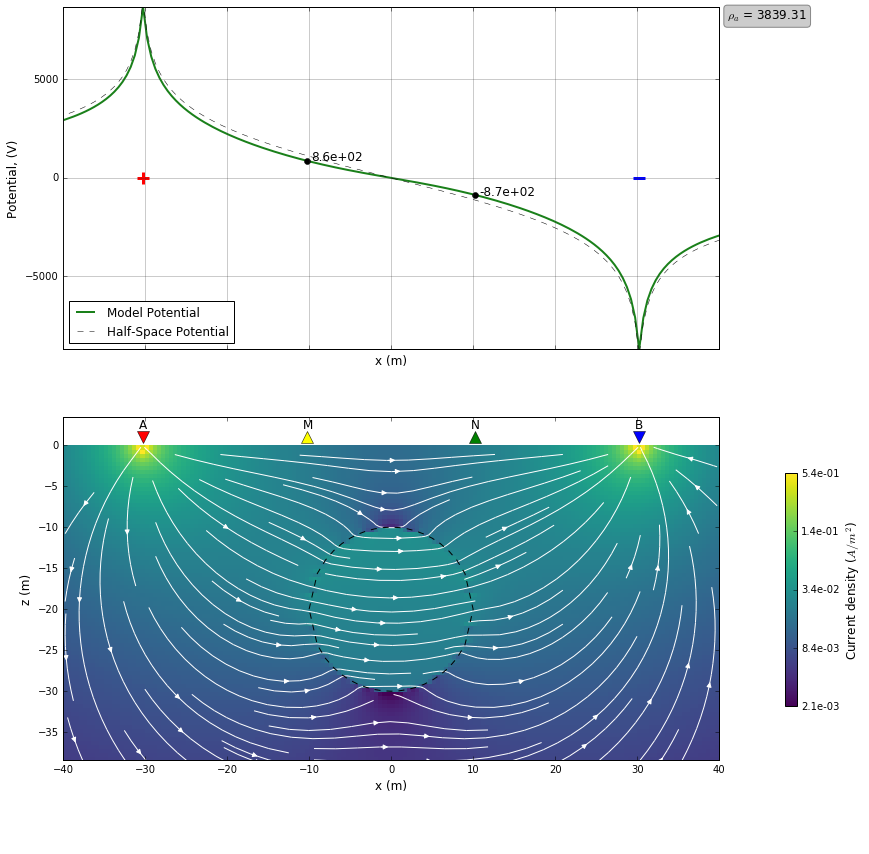
\includegraphics[width=.9\linewidth]{figures/DC_survey.png}
  \captionof{figure}{DCR potential field at the surface and underground current flow}
  \label{DC_pot_fields}
\end{minipage}
\end{figure}

\newpage
Maxwell's equation forms a complex system of Partial Differential Equations. In most cases, there is no analytic solution except for very simple problems (half-space, sphere in void…). To forward model the response of complex structures, numerical techniques are required. We are using for this project the Python open-source package SimPEG (\cite{CKH+:2015}) for the forward modeling of DCR data and perform L2-regularized inversions.

L2-regularized inversions is the most widely used type of inversions for diffusive electromagnetic and potential fields geophysics with a high rate of success (\cite{Haber:2014}). Recovered models using this type of inversion are smooth, which is compliant with the diffusive nature of the physics but not with the sharp geological contacts that are usually expected. Some progress have been made recently for potential fields inversions using L1-regularized inversions, through it needed implementations of Ad Hoc strategies (\cite{Fournier:2015}).  

Compressive Sensing is a popular topic in signal processing first introduced in (\cite{CRT:2006}). It aims at recovering sparse approximations of a signal in a transformed space from less measurements than required by the Shannon-Nyquist sampling theorem. its keys ideas are first to use a sparsifying transform to the model parameters and then work in this sparsifying space, second to generate coarse randomized sampling in the sparsifying domain, and at last to use a sparsity-promoting solver to recover a sparse approximations.

Despite being first thought for frequency measurements in (\cite{CRT:2006}), we propose in this project to apply some of these ideas to a static electromagnetic geophysics example. Random subsampling in DCR have been used in the past as for example in the DCR inversion with simultaneous sources case presented in (\cite{HCH:2012}) to reduce the number of right-hand sides. We will apply a similar stochastic approach to our case and present the impact of several strategies for the choices of the random matrix in term of its nature, size and updates. We will then promote sparsity in a transform space in the Gauss-Newton subproblems of the inversion both in the deterministic and stochastic formulation and compare the results. For this purpose we will be using the SPGl1 package presented in (\cite{BF:2008}).

To ensure the reproducibility of this work, scripts to re-create most of the results generated for this project are available through Github at the address: https://github.com/thast/EOSC513

%------------------------------------------------

\newpage
\section{the DCR method}

The formulation of the DCR problem and its discretization in finite volume have been done with extensive details in (\cite{CHO:2016}). We are reproducing here some of theirs visuals (figure \ref{DCequations}).


%\vspace{-10pt}
\begin{figure}[!ht]
\centering
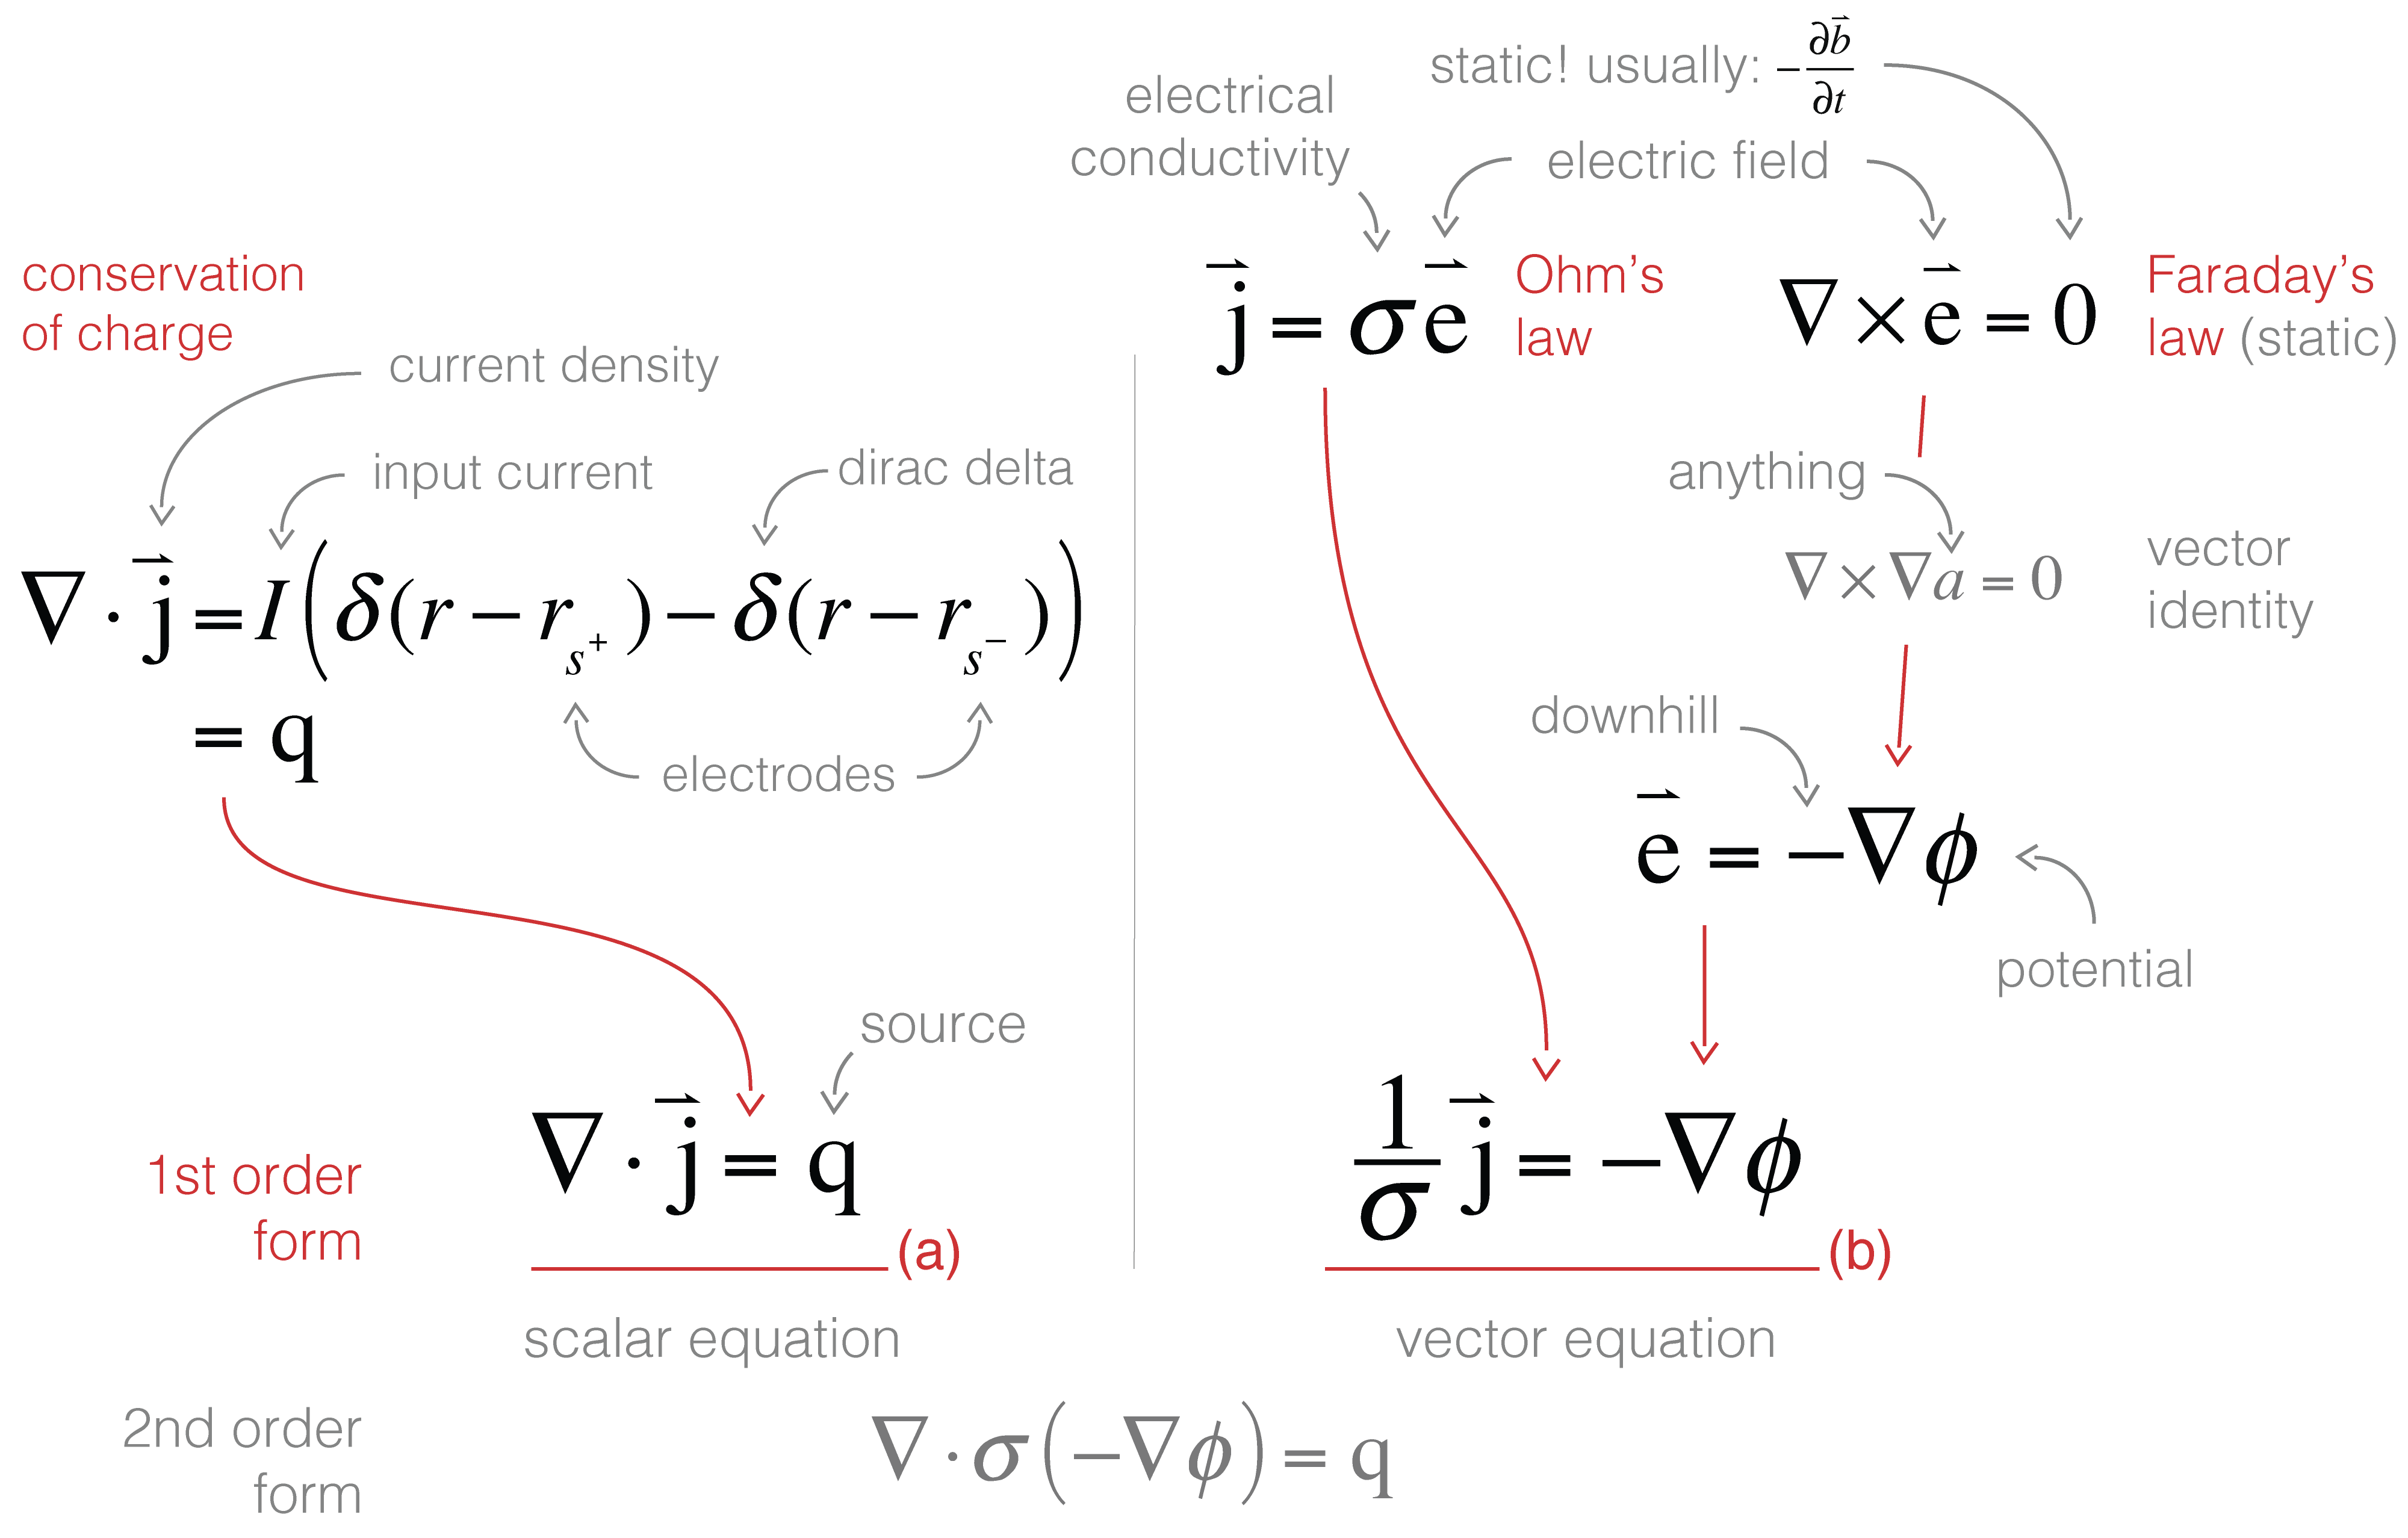
\includegraphics[width=.55\linewidth]{figures/DCEquations.png}
\caption{From Maxwell's equations to DC resistivity problem}
\label{DCequations}
%\vspace{-40pt}
\end{figure}

Assuming Neumann boundaries conditions, we obtain the discretization of the DCR equation described in figure \ref{DCequations} in finite volume (\cite{CHO:2016}): 
\begin{align}
\text{diag}(\mathbf{v}) \mathbf{D} \mathbf{M}_f(\sigma^{-1})^{-1} \mathbf{D}^\top \text{diag}(\mathbf{v}) \boldsymbol{\phi} &= \mathbf{q} \\
A(m) \phi &= q \label{DC_fields}
\end{align}

With $\mathbf{D}$ the Divergence operator, $\mathbf{v}$ a vector containing the cells volume, and $\mathbf{M}_f(\sigma^{-1})^{-1}$ a weighted averaging operator from cells center to faces (see \cite{CHO:2016} and \cite{Haber:2014}). the model $m$ is usually chosen as the log of the electrical conductivity, $m = ln(\sigma)$ to ensure the positivity of the recovered conductivity during the inversion process.

In a typical DCR survey, electrodes will be layout on a regular grid. Data will be acquired for several sequential sources. As a rule of thumb, the more spacing there is between the two sources electrodes, the deeper you investigate. Using several sources with different positions and spacing then give us information at several locations and depths.
For several sources, the equation \ref{DC_fields} can be written as:
\begin{align}
\text{for all sources $q_i$: } A(m) \phi_i &= q_i \\
\text{or }A(m)\Phi &= Q \label{DC_SimSrcs}
\end{align}

With:
\begin{align}
Q = 
\left[
  \begin{array}{cccc}
    \vertbar & \vertbar &        & \vertbar \\
    q_{1}    & q_{2}    & \ldots & q_{N_s}    \\
    \vertbar & \vertbar &        & \vertbar 
  \end{array}
\right]
\text{ and }&
\Phi = 
\left[
  \begin{array}{cccc}
    \vertbar & \vertbar &        & \vertbar \\
    \phi_{1}    & \phi_{2}    & \ldots & \phi_{N_s}    \\
    \vertbar & \vertbar &        & \vertbar 
  \end{array}
\right]
\end{align}

and the observed data can be express as: 
\begin{align}
\text{for all sources $q_i$: } d_i = PA(m)^{-1}q_i \label{data} \\
\text{or }D = PA(m)^{-1}Q \label{DC_SimSrcs_2}
\end{align}
With $P$ the projection matrix from the electric potential fields $\phi$ to the receivers electrodes.

The matrix formulation presented in equations \ref{DC_SimSrcs} and \ref{DC_SimSrcs_2} will be useful at the conceptual level for formulating the simultaneous sources problem.

To learn more about the DCR method, We invite the reader to take a look at the website \href{http://em.geosci.xyz/content/geophysical_surveys/dcr/index.html}{em.geosci} developed at the University of British Columbia.

\section{L2-Regularized Inversion}

To reconstruct a model from observed data, we need to define an objective-function for our inversion problem. For DCR, the usual objective-function is:
\begin{align}
%f(m) &= \frac{1}{2} \sum_{i=1}^{N_s} ||P_iA(m)^{-1}q_i-d_i||_2^2 + \frac{\beta}{2} ||W(m-m_{ref})||_2^2 \\
%f(m) & = \frac{1}{2} ||PA(m)^{-1}Q-D||_F^2  + \frac{\beta }{2} ||W(m-m_{ref})||_2^2 \\
f(m) &= \frac{1}{2} ||d(m)-d_{obs}||_2^2 + \frac{\beta }{2} ||R(m-m_{ref})||_2^2 \label{objectiveFunction}
\end{align}

With $d_{obs}$ a vector containing our observed data and $d(m)$ a vector containing our modeled data with equation \ref{data}, the first term represents the data fitting objective. The second term is a Tikhonov-style regularizer (\cite{Tik:1977}) that contains a-priori information about the model, such as the reference model $m_{ref}$.The matrix $R$ usually includes the Identity for smallness and first or higher order gradients for directional smoothness. $\beta$ is the regularizer's weight. This term is iteratively cooled down during the inversion process, giving more and more weights to the data fitting term. Our goal is then to find a model $m$ that minimize the value $f$. As this is an underdetermined nonlinear problem, an iterative scheme is use to solve this optimization problem. We look for an update $\delta m$ such that we decrease enough the objective-function value:

\begin{align}
f(m+\delta m) &= \frac{1}{2} ||r(m+ \delta m)||_2^2 + \frac{\beta }{2} ||W(m+ \delta m-m_{ref})||_2^2 \label{LinearizedObjFunc}\\
\text{s.t. } f(m+\delta m) & \leq \gamma f(m) \text{ with } \gamma \geq 1 \\
\text{With the residual: }  r(m) &= d(m)-d_{obs}
\end{align}

To solve this problem, we first linearize the system:
\begin{align}
f(m+\delta m) &= \frac{1}{2} ||r(m)+J(m)\delta m||_2^2 + \frac{\beta }{2} ||W(m+\delta m-m_{ref})||_2^2 \label{linearized_DCproblem}
\end{align}

With $J$ the Jacobian matrix of the data residual $r$ (\cite{Haber:2014}).

We then obtain by derivation the Gauss-Newton system, whose solution gives us the Gauss-Newton update $\delta m$: 
\begin{align}
H \delta m &= -g \\
\text{With: } H = &J^TJ+\beta W^TW \\
\text{and: } g &= J^Tr(m) + \beta W^TW(m-m_{ref})
\end{align}

We finally update our previous model $m_k$ with an additional line search
\begin{align}
m_{k+1} = m_k+\alpha \delta m \text{ s.t. } f(m_{k+1}) < \gamma f(m_{k}) \text{ with } \gamma \geq 1
\end{align}

\begin{figure}[t!]
    % \begin{center}
    \centering
    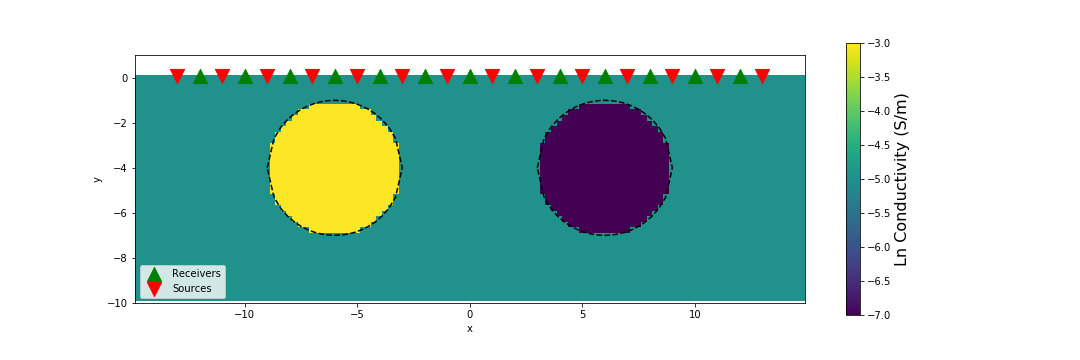
\includegraphics[width=0.8\linewidth]{figures/initialmodel.png}
    \caption{Initial model and survey}
    \label{InitialModel}
    % \end{center}
\end{figure}

  
\begin{figure}[t!]
    % \begin{center}
    \centering
    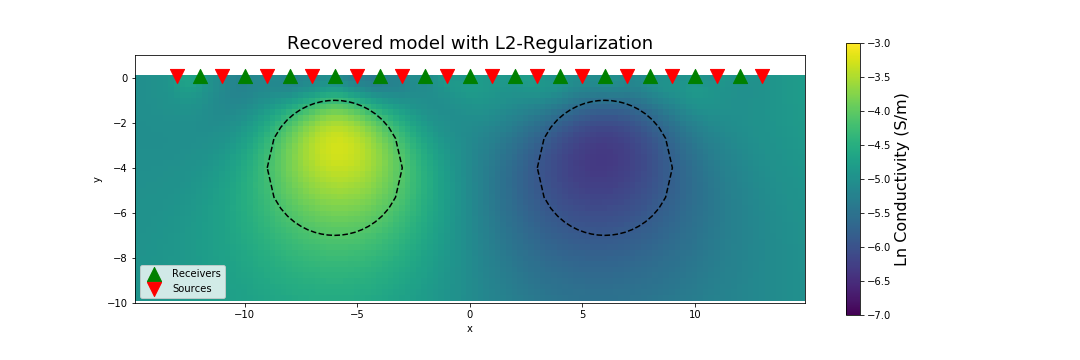
\includegraphics[width=0.8\linewidth]{figures/recoveredModel.png}
    \caption{Recovered model with L2 Regularization}
    \label{L2Model}
    % \end{center}
\end{figure}

We applied this scheme to an toy example problem (figure \ref{InitialModel}). This example is composed of 23 dipoles sources of various length. Every sources share the same dipoles receivers for a total of 276 measurements. The recovered model is presented in figure \ref{L2Model}. The overall position and polarity of the anomalies is well recovered but, as expected, the result is quite smooth and it is hard to get a precise idea of the initial shapes.

We will then try to use some ideas from Compressive Sensing to our case to sparsify the recovered model in a transform space that might improve the anomalies locations and values in the recovered models.

\newpage

\section{Basics ideas of Compressive Sensing}

The first goal of Compressive Sensing is to solve the underdetermined linear problem:
\begin{align}
\min_x ||x||_0 \text{ s.t. } Ax=b  \label{CompressiveSensing}
\end{align}

Compressive Sensing theory is telling us that if $A$ is an incoherent matrix and $x$ is sparse, $x$ can be recovered exactly under certain conditions. If the original $x$ is not sparse but can be represent sparsely in some transform space through a linear transform $S$, we can rewrite the original problem \ref{CompressiveSensing} as:

\begin{align}
\min_x ||x||_0 \text{ s.t. } RMS^Hx=b
\end{align}

with $S$ the sparsifying transform, $M$ the measurement matrix and $R$ the restriction matrix. According to Compressive Sensing theory, We need the rows of M and S to be incoherent, which means their inner-products are small. However this is still an NP-hard problem. \cite{CRT:2006} showed that, under certain conditions, the L1 minimization problem (equation \ref{CompressiveSensingL1}) can still recover a robust approximation of $x$, with less measurements than required by the Shannon-Nyquist sampling theorem by using coarse randomized sampling in the sparsifying domain.

\begin{align}
\min_x ||x||_1 \text{ s.t. } RMS^Hx=b  \label{CompressiveSensingL1}
\end{align}

In the following project, we have used the SPGl1 package (\cite{BF:2008}) to solve the problem presented in equation \ref{CompressiveSensingL1}

\newpage

\section{Simultaneous Sources}

We first started by investigating random simultaneous sources in the case of DCR survey. We can formulate the inverse problem shown in equation \ref{objectiveFunction} as a stochastic problem, following the work done in (\cite{HCH:2012}), by randomly mixing the original sources into a smaller number of simultaneous sources. Reducing the number of sources can make computing the Gauss-Newton update much computationally efficient as for each step we need to solve $2N_s$ Partial Differential Equations systems, with $N_s$ the number of sources. We generate the random simultaneous sources following: 

\begin{align}
f(m) & = \frac{1}{2} ||PA(m)^{-1}QW-DW||_F^2  +\beta R(m) \label{stochastic}
\end{align}

With $W$ a random Gaussian or Rademacher matrix of size $N_s \times N_{ss}$ with $N_{ss}<<N_s$, $N_{ss}$ being the number of final recombined sources and $N_s$ the original number of sources.
The Gauss-Newton step subproblem's size is then reduced by a factor $\frac{N_{s}}{N_{ss}}$

\begin{figure}[!ht]
\centering
\begin{minipage}{0.49\textwidth}
  \centering
    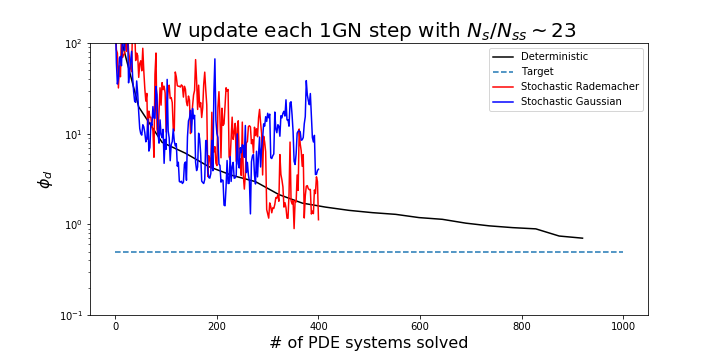
\includegraphics[width=.99\linewidth]{figures/W_update_each_1GN_steps_with_1_sources.png}
  \captionof{figure}{Reduction to 1 source, \\ update W each GN step}
  \label{1S1GN}
\end{minipage}%
\begin{minipage}{.49\textwidth}
  \centering
  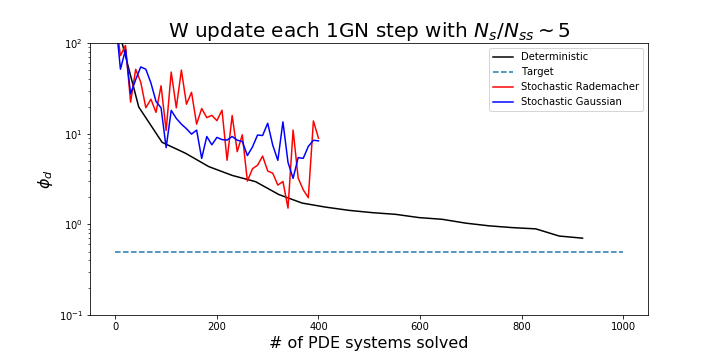
\includegraphics[width=.99\linewidth]{figures/W_update_each_1GN_step_with_5_sources.png}
  \captionof{figure}{Reduction to 5 sources, \\ update W each GN step}
  \label{5S1GN}
\end{minipage}
\begin{minipage}{.49\textwidth}
  \centering
  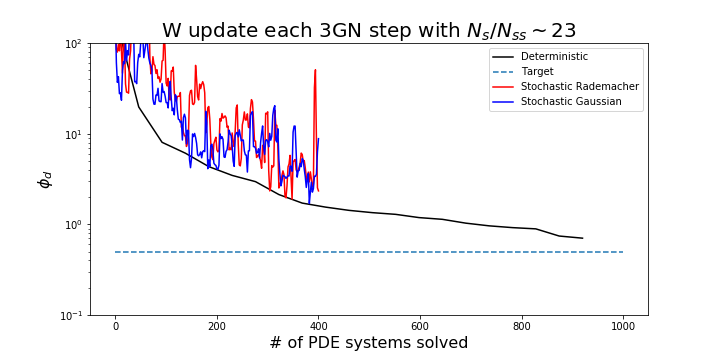
\includegraphics[width=.99\linewidth]{figures/W_update_each_3GN_step_with_1_source.png}
  \captionof{figure}{Reduction to 1 source, \\ update W each  3 GN step}
  \label{1S3GN}
\end{minipage}
\begin{minipage}{.49\textwidth}
  \centering
  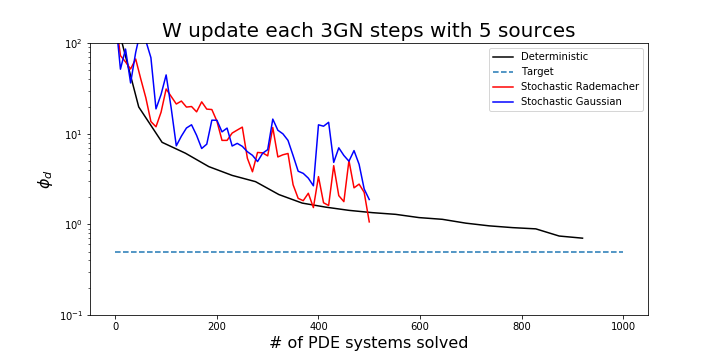
\includegraphics[width=.99\linewidth]{figures/W_update_each_3GN_steps_with_5_sources.png}
  \captionof{figure}{Reduction to 3 sources, \\ update W each  3 GN step}
  \label{5S3GN}
\end{minipage}

\end{figure}

Without any update to W during the inversion process, we have seen that we converge to a local minima but that the recovered model, when compared to the full data set, still present a very high misfit. We have then experiment several strategies for updating W (figure \ref{1S1GN}, \ref{5S1GN}, \ref{1S3GN}, \ref{5S3GN}) and their effects on the convergence rate for the data misfit. The parameter $\beta$ was still cooled down to mimic the strategy used during the deterministic inversion. The different graphs represent the data misfit of the model recovered after each Gauss-Newton step compared to the whole data set, not the simulated data obtained through the simultaneous sources. We represent in blue the tests with Gaussian matrix, in red the tests with Rademacher matrix and in black the deterministic case. The dashed line indicates the misfit target based on the noise level of the data. We observe that taking a Gauss-Newton step on a particular realization of a simultaneous sources does not guarantee that this will decrease the misfit with the overall dataset. However we can see that the stochastic curves roughly follow the trend of the deterministic case.  As expected, the convergence curves obtained when we less reduce the number of sources (going from 23 original sources to 5 instead of just 1) are smoother and closer to the deterministic case.


\begin{figure}[t!]
    % \begin{center}
    \centering
    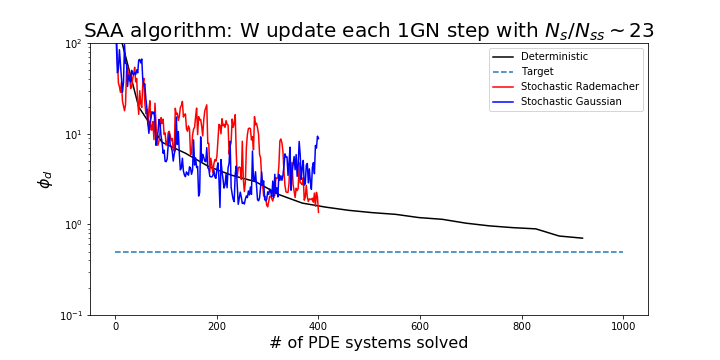
\includegraphics[width=0.5\linewidth]{figures/SAA_algo.png}
    \caption{SA algorithm: Keep in memory the previous update}
    \label{SAA}
    % \end{center}
\end{figure}

We also took a look at a stochastic algorithm that keep in memory the previous updates, as presented in (\cite{HCH:2012}) (figure \ref{SAA}), named Stochastic Approximation (SA). We can observe that this improves slightly the behavior of the convergence curves compared to figure \ref{1S1GN} but the same flows are still present.
It is very likely that our test example is too small to benefit from such an approach. It is also possible that, as we are in a static case and thus dealing with potential fields, that the random mixing of these fields create unexpected patterns, emphasizing much more the sensitivity of certain areas over others that get masked.

Overall we would only recommend using this approach for huge dataset for which computing the Gauss-Newton update based on the full original dataset would not be possible memory-wise and with better chance to have redundant data. 

\section{Promoting Sparse Gauss-Newton update}

In this section, we are aiming at solving system similar to equation \ref{CompressiveSensingL1} defined by Compressive Sensing using the SPGl1 solver \cite{BF:2008}. 

\subsection{Formulating the subproblem}

We can rewrite our original linearized problem from equation \ref{linearized_DCproblem} in a similar form than in equation \ref{CompressiveSensingL1}  without the L2 penalty but a L1 constrain in some sparsifying domain:

\begin{align}
\text{min} ||\delta x||_1 ~\text{s.t}~ & ||J(m)S^H \delta x + r(m)||^2_2 < \tau \label{SparseGN}
\end{align}

With

\begin{align}
\delta x &= S \delta m
\end{align}

Note that if we still have additional information such as a good reference model or weights, we can still add it as an L2 term in the above formulation. Bounds on the physical properties are also possible, through it would present its own challenge to implement it successfully.

\newpage

\subsection{Choosing a sparsifying transform}

\begin{figure}[H]
  \centering
  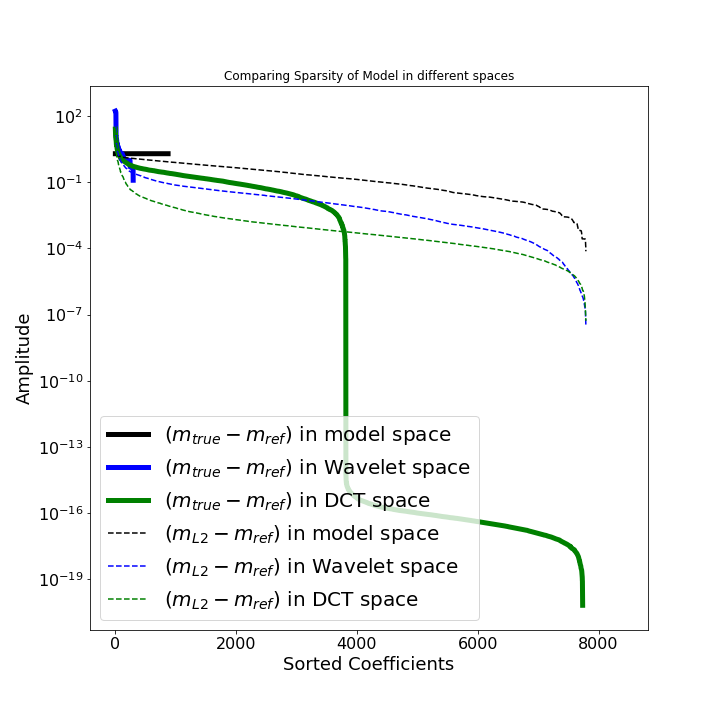
\includegraphics[width=0.35\linewidth]{figures/Model_sparsity_diff_spaces.png}
  \caption{Sparsity of the true model (plain) and recovered model (dashed) (minus reference model) in different spaces}
  \label{Sparsity_model}
\end{figure}

\begin{figure}[!ht]
\centering
\begin{minipage}{0.31\textwidth}
  \centering
    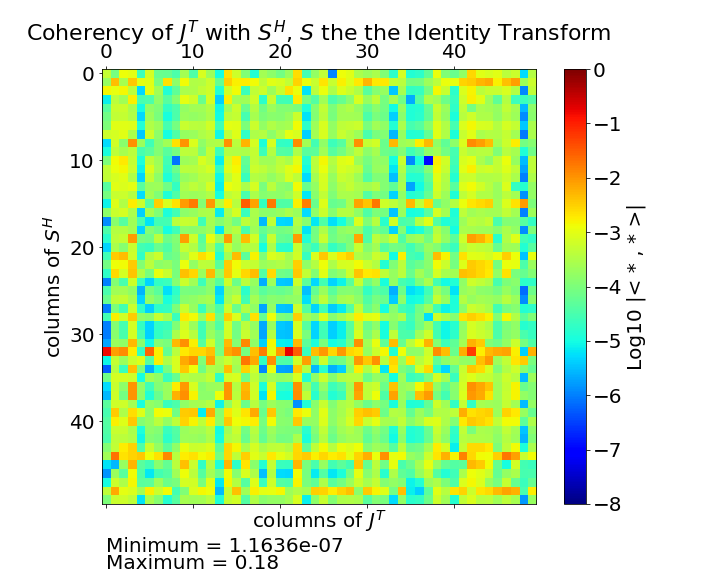
\includegraphics[width=.99\linewidth]{figures/Coherency_Identity.png}
  \captionof{figure}{Coherency \\$J^T$ with Identity}
  \label{Coh_Id}
\end{minipage}%
\begin{minipage}{.31\textwidth}
  \centering
  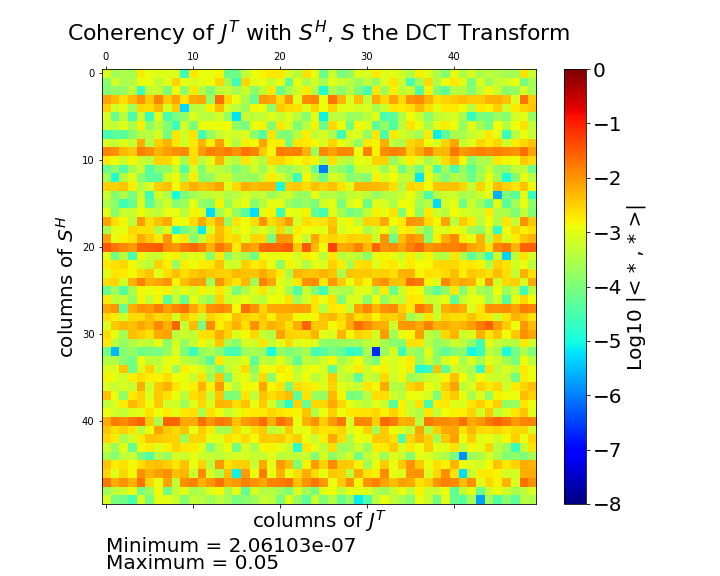
\includegraphics[width=.99\linewidth]{figures/Coherency_DCT.png}
  \captionof{figure}{Coherency \\J$^T$ with DCT}
  \label{Coh_DCT}
\end{minipage}
\begin{minipage}{.31\textwidth}
  \centering
  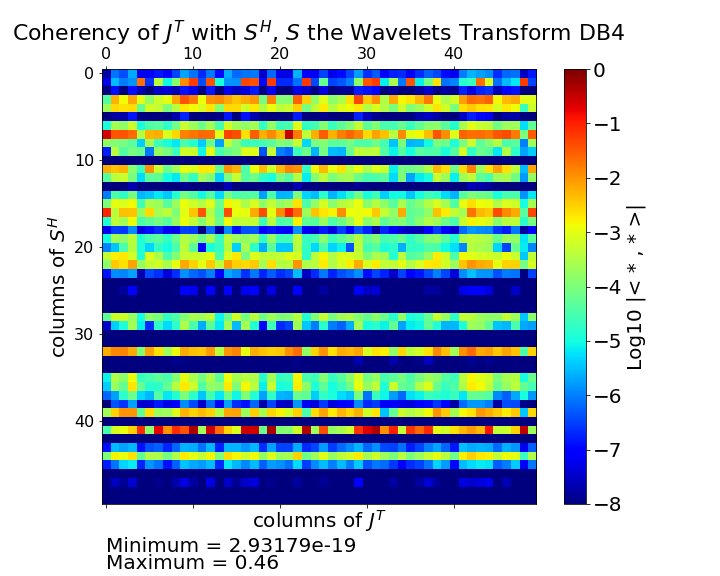
\includegraphics[width=.99\linewidth]{figures/Coherency_WaveletDB4.png}
  \caption{Coherency \\$J^T$ with the WVT4}
  \label{Coh_DB4}
\end{minipage}
\end{figure}

Based on classic Compressive Sensing, choosing the sparsifying transform requires two conditions. First the model we are trying to recover can be decompose or at least approximate by a sparse representation in the chosen space (figure \ref{Sparsity_model}). Second, to ensure some guarantee on the quality of the recovery, the columns of $J^T$ and $S^H$ in equation \ref{SparseGN} should be incoherent.

We choose here to test the Identity transform (no transform), because this is in the end the domain of interest. We also tested the Direct Cosine Transform (referred later as DCT), as the DCR problem is a weighted Laplacian and that the eigenfunctions of a Laplacian are cosine and sine functions. Intuitively it then seems that just a few coefficients in this space should be able to explain the data. Finally we tested the 4th order Daubechies wavelet transform (WVT4) as a compromise between localized but still smooth model update. We also tested the lower orders wavelet transforms but we got our best results with the 4th order ones.

Based on figure \ref{Sparsity_model},from the true model point of view, both Identity and Wavelet seem like potential candidates for $S$ while the DCT do not help much sparsifying the model. 
From the DCR Jacobian point of view, the DCT presents the most constant and lowest maximum of coherency (figure \ref{Coh_DCT}). This was expected, for the reasons mentioned above. Interestingly, the WVT4 present a lot of very small coherency coefficients with few very high coefficients (figure \ref{Coh_DB4}). The Identity transform presents an almost uniform coherency that is fairly higher than the DCT but lower than the maximum for the WVT4 (figure \ref{Coh_Id}).

\newpage

\subsection{Recovered models}

We compare here the models obtained by using different sparsifying transform such as discussed in the previous subsection.

\begin{figure}[!ht]
\centering
\begin{minipage}{0.99\textwidth}
  \centering
    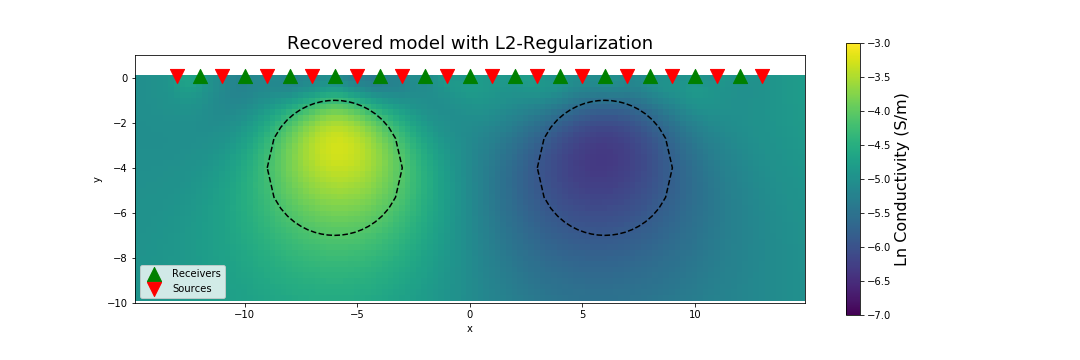
\includegraphics[width=.75\linewidth]{figures/recoveredModel.png}
  \captionof{figure}{Recovered model with L2 regularization}
  \label{recoveredModel_L2}
\end{minipage}
\begin{minipage}{.99\textwidth}
  \centering
  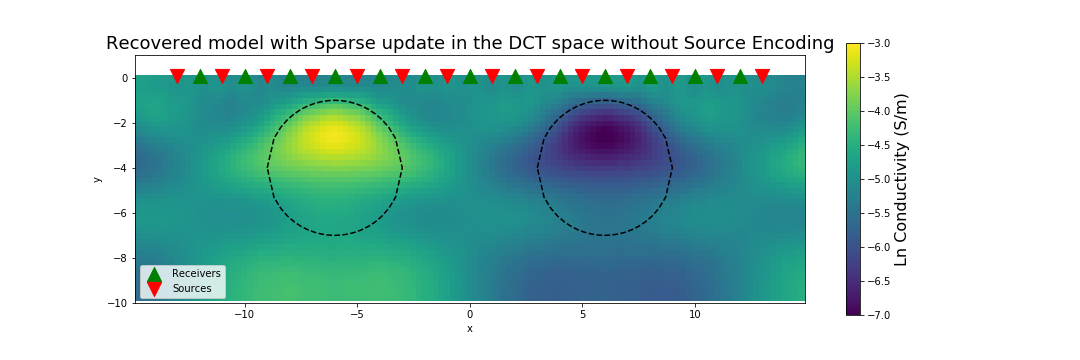
\includegraphics[width=.75\linewidth]{figures/recoveredModel_SparseDCT.png}
  \captionof{figure}{Recovered model with DCT as $S$}
  \label{recoveredModel_DCT}
\end{minipage}
\begin{minipage}{.99\textwidth}
  \centering
  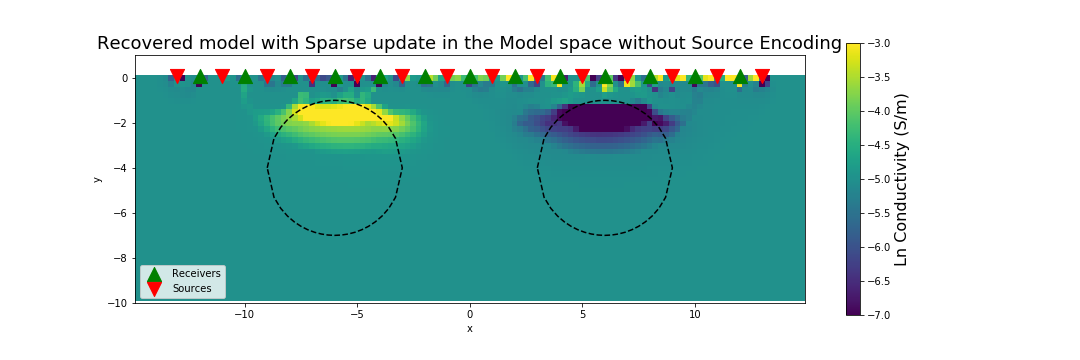
\includegraphics[width=.75\linewidth]{figures/recoveredModel_SparseId.png}
  \captionof{figure}{Recovered model with Identity as $S$}
  \label{recoveredModel_Id}
\end{minipage}
\begin{minipage}{.99\textwidth}
  \centering
  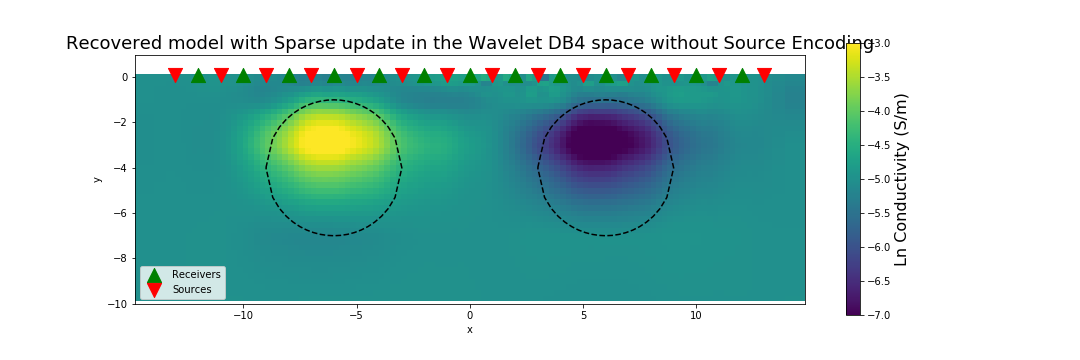
\includegraphics[width=.75\linewidth]{figures/recoveredModel_SparseWVT_DB4_withoutW.png}
  \captionof{figure}{Recovered model with WVT4 as $S$}
  \label{recoveredModel_WVT4}
\end{minipage}
\end{figure}

\newpage

Interestingly, each model are quite different and reach (or close to reach) the target data misfit (figure \ref{Convergence}).

For the sparse GN update in the model space (Identity transform), SPGl1 got more difficulties to solve the problem (figure \ref{Convergence}) and each iteration took a long time to compute compared to update in other spaces. The recovered model (figure \ref{recoveredModel_Id}) is quite compact but noisy. When looking at the updates, even without simultaneous sources, we realize these updates are not that sparse (figure \ref{Sparsity_ID}).

For the sparse GN updates in the DCT space (DCT transform), SPGl1 reach the target misfit in just few GN steps (figure \ref{Convergence}), which we can relate to the small coherency between of $J$ and $S$. The recovered model still displays the periodicity of the basis function, which has nothing to do with the true model (figure \ref{recoveredModel_DCT}).

Finally, despite a few high coherency coefficients between $J$ and $S$, the Wavelet transform with 4th order Daubechies wavelets gave us a satisfying result, both in term of the number of iterations to reach the target data misfit (figure \ref{Convergence}) and in term of the recovered model (figure \ref{recoveredModel_WVT4}). The recovered model is still smooth but anomalies are must less spread out compared to the L2-regularized model. The recovered physical properties are also much closer to those of the true model.

We do not have a definite answer to why the wavelet transform works that well despite some high-coherency coefficients. A hypothesis to test would be to evaluate if our Jacobian $J$ and the wavelet transform are "asymptotically incoherent" instead of fully incoherent. Under this conditions, it has been shown recently that most of the Compressive Sensing results still hold (\cite{A2017}).

\begin{figure}[H]
    % \begin{center}
    \centering
    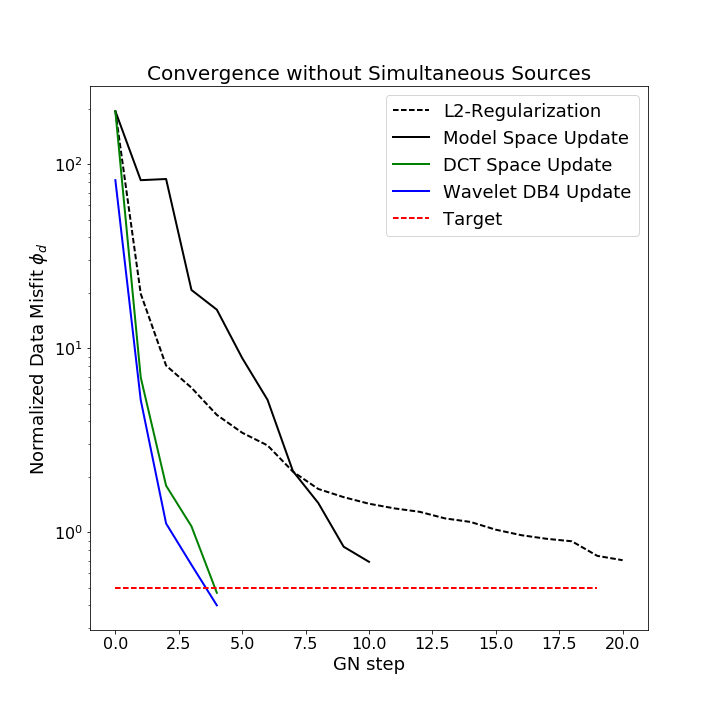
\includegraphics[width=0.4\linewidth]{figures/Convergence_Sparse_withoutW.png}
    \caption{Convergence of the data misfit for each type of Gauss-Newton update}
    \label{Convergence}
    % \end{center}
\end{figure}

\subsection{Sparse Gauss-Newton update with Simultaneous Sources}

\begin{figure}[!ht]
\centering
\begin{minipage}{.31\textwidth}
  \centering
  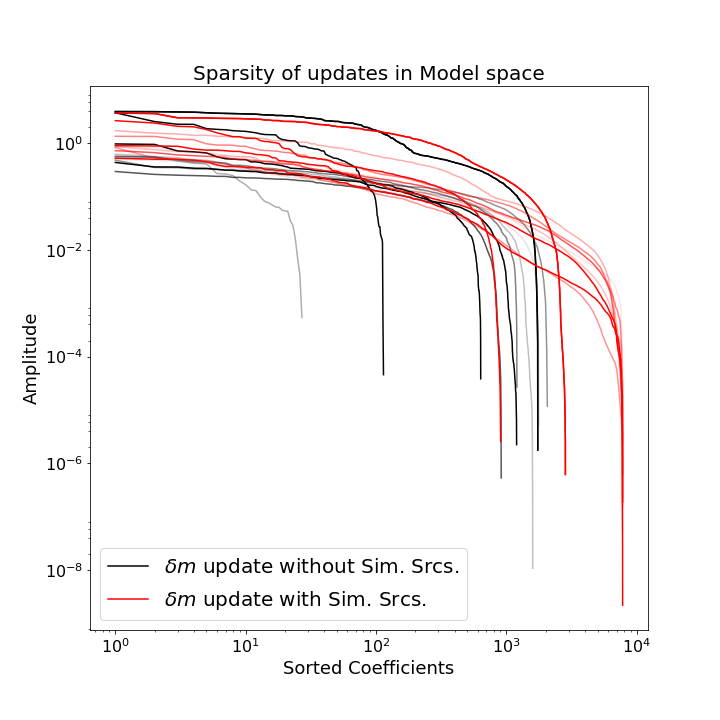
\includegraphics[width=.99\linewidth]{figures/SimSrc_kills_Sparsity_Id.png}
  \captionof{figure}{Sparsity of updates with Identity as $S$}
  \label{Sparsity_ID}
\end{minipage}
\begin{minipage}{.31\textwidth}
  \centering
  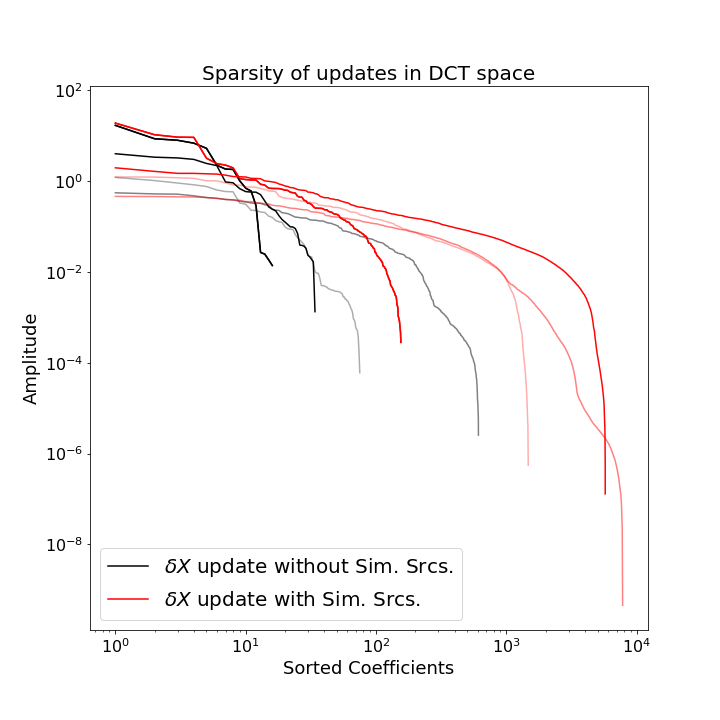
\includegraphics[width=.99\linewidth]{figures/SimSrc_kills_Sparsity_DCT.png}
  \captionof{figure}{Sparsity of update with DCT as $S$}
  \label{Sparsity_DCT}
\end{minipage}
\begin{minipage}{0.31\textwidth}
  \centering
    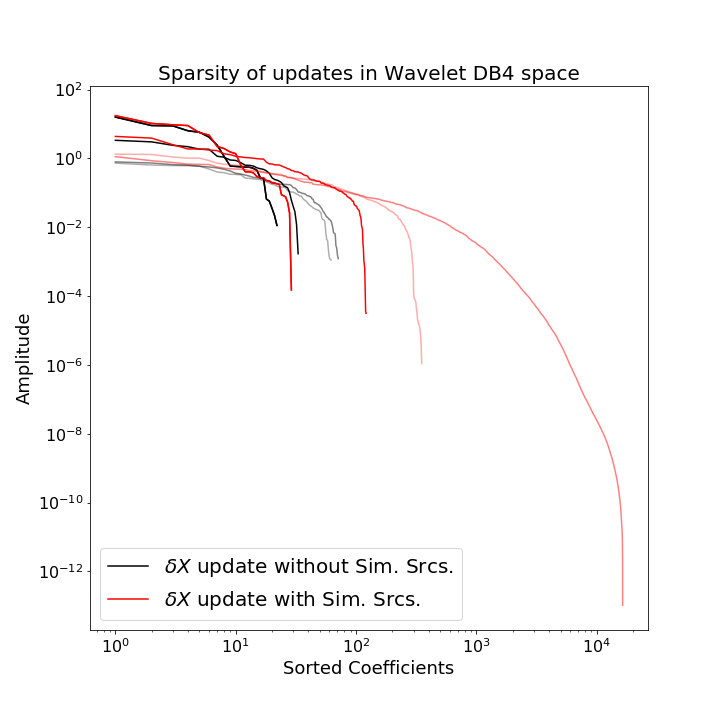
\includegraphics[width=.99\linewidth]{figures/SimSrc_kills_Sparsity_WVT_DB4.png}
  \captionof{figure}{Sparsity of updates with WVT4 as $S$}
  \label{Sparsity_WVT4}
\end{minipage}
\end{figure}

In this section, we present to the audience an unexpected problem we encountered while combining the sparse Gauss-Newton update approach with the simultaneous sources. Our expectation would have been that, as when we are decreasing the number of sources we are also decreasing the available information at each iteration, this would also simplifies sparsifying the update. What happened is the exact opposite. By mixing the sources together into a smaller number of final sources, SPGl1 became much slower to solve each subproblem. Worse, the updates where no longer sparse anymore, or not as sparse as before, whatever transformed we used (figure \ref{Sparsity_ID}, \ref{Sparsity_DCT}, \ref{Sparsity_WVT4}).
For now, one possible explanation refers back to the discussion about the simultaneous sources results, that our example might be too small to use a stochastic approach or unevenly highlight certain areas over others.

\section{Discussion and Conclusion}

The tests we performed on our toy example for simultaneous sources have shown a similar or worse rate of convergence, in term of number of PDE systems solved, compared to using the full system in a deterministic process. However each step is a lot less memory-expansive, making it useful if yours systems are too big to be efficiently stored. It is possible that we may have obtained better results on a larger example with more redundancy of information in the acquired data. When used in combination with the sparse update approach, simultaneous sources have make things very difficult for SPGl1 to solve, in reverse to our initial intuition that decreasing the level of information would make the update easier and sparser.

At first, it seemed we had an antagonization for choosing a sparsifying transform that both allows a sparse representation of the expected model and that is incoherent with the Jacobian of the DCR problem. The Direct Cosine Transform was appropriate with the diffusive nature of the physics but did not allow a good reconstruction of the model. An identity transform was not enough incoherent to be efficiently solved and to ensure the quality of the reconstruction. Finally, a 4th order Daubechies wavelet transform seemed to be able to bridge the gap between the model and the physics by allowing smooth but very localized model updates despite some very high coherent coefficients with the DCR Jacobian. Our hypothesis to explain why the wavelet transform is working is that it may be asymptotically incoherent with the DCR Jacobian, which would still be a sufficient condition to preserve the properties of Compressive Sensing.

We did not study the influence of the $\tau$ parameter for the data fitting term in SPGL1 or the strategy to set it. The few tests we performed did not seem to change much the final recovered model but only the number of Gauss-Newton updates to reach the desired target data misfit and the time necessary to compute each of the update. The smaller $\tau$ was, the fewer Gauss-Newton steps was needed but each step was more expansive to compute. There could be then an ideal value that optimize the time taken by the inversion but it could be highly problem-specific.

Finally, to ensure the reproducibility of this work, scripts to re-create most of the results generated for this project are available through Github at the address: https://github.com/thast/EOSC513

\section{Acknowledgments}
We would like to thanks Seogi Kang and Devin Cowan, all students at UBC - Geophysical Inversion Facility for sharing theirs experiences during the making of this project.
%----------------------------------------------------------------------------------------
%	REFERENCE LIST
%----------------------------------------------------------------------------------------
\newpage

\begin{thebibliography}{99}

\bibitem{A2017}
Adcock, Ben, et al. (2017)
\newblock "Breaking the coherence barrier: A new theory for compressed Sensing." Forum of Mathematics, Sigma. Vol. 5. Cambridge University Press, 2017.

\bibitem{BF:2008}
Berg E. van den  and Friedlander M. P. (2008)
\newblock "Probing the Pareto frontier for basis pursuit solutions", SIAM J. on Scientific Computing, 31(2):890-912, November 2008

\bibitem{CRT:2006}
Candes E., Romberg J., Tao T. (2006)
\newblock "Robust Uncertainty Principles: Exact Signal Reconstruction from Highly Incomplete Frequency Information"
\newblock IEEE Trans. Inform. Theory, 52(2): 489-509

\bibitem{CHO:2016}
Rowan Cockett, Lindsey J. Heagy, and Douglas W. Oldenburg (2016)
\newblock ”Pixels and their neighbors: Finite volume.” The Leading Edge, 35(8), 703–706. doi: 10.1190/tle35080703.1
\newblock http://tutorials.simpeg.xyz/content/pixelsandtheirneighbors.html

\bibitem{CKH+:2015}
Cockett, Rowan, Seogi Kang, Lindsey J. Heagy, Adam Pidlisecky, and Douglas W. Oldenburg (2015)
\newblock "SimPEG: An Open Source Framework for Simulation and Gradient Based Parameter Estimation in Geophysical Applications." 
\newblock {\em Computers and Geosciences}, September 2015. doi:10.1016/j.cageo.2015.09.015.

\bibitem{Fournier:2015}
Fournier D. (2015)
\newblock A cooperative magnetic inversion method with Lp-norm regularization, M.Sc. Thesis

\bibitem{Haber:2014}
Haber E.(2014).
\newblock "Computational Methods in Geophysical Electrodynamics"

\bibitem{HCH:2012}
E. Haber, M. Chung, and F. Herrmann (2012)
\newblock  “An Effective Method for Parameter Estimation with PDE Constraints with Multiple Right-Hand Sides,” SIAM Journal on Optimization, vol. 22, no. 3, pp. 739–757, jul 2012.

\bibitem{HCK:2016}
Heagy J. lindsey, Rowan Cockett, Seogi Kang, Gudni K. Rosenkjaer, Douglas W. Oldenburg (2016)
\newblock "A framework for simulation and inversion in electromagnetics"
\newblock {\em Geophysics}

\bibitem{Pardiso1}
Luisier M. , O. Schenk et.al. (2013)
\newblock Fast Methods for Computing Selected Elements of the Green's Function in Massively Parallel Nanoelectronic Device Simulations
\newblock Euro-Par 2013, LNCS 8097, F. Wolf, B. Mohr, and D. an Ney (Eds.), Springer-Verlag Berlin Heidelberg, pp. 533–544, 2013.

\bibitem{Pardiso2}
Schenk O., M. Bollhöfer, and R. Römer,
\newblock On large-scale diagonalization techniques for the Anderson model of localization.
\newblock Featured SIGEST paper in the SIAM Review selected "on the basis of its exceptional interest to the entire SIAM community". SIAM Review 50 (2008), pp. 91-112.

\bibitem{Pardiso3}
Schenk O., A. Wächter, and M. Hagemann,
\newblock Matching-based Preprocessing Algorithms to the Solution of Saddle-Point Problems in Large-Scale Nonconvex Interior-Point Optimization.
\newblock Journal of Computational Optimization and Applications, pp. 321-341, Volume 36, Numbers 2-3 / April, 2007.

\bibitem{SEG:2016}
Society of Exploration Geophysicists
\newblock Reproducible research: Geophysics papers of the future 2016
\newblock http://library.seg.org/page/Geophysics/reproducible-research:-geophysics-papers-future?mobileUi=0

\bibitem{Telford}
Telford, W.M., Geldart, L.P. and Sheriff, R.E. (1990)
\newblock Applied Geophysics, 2nd Edition: Cambridge University Press, 1990.

\bibitem{Tik:1977}
Tikhonov, A.N., Arsenin, .V.Y. (1977)
\newblock "Solution of Ill-posed problems", Winston and Sons, Washington, 1977  

\bibitem{WH:1988}
S. H. Ward, C. W. Hohmann (1988).
\newblock "Electromagnetic Theory for Geophysical Applications", in Nabighian, M. N., Ed., Electromagnetic Methods in Applied Geophysics: Society of Exploration Geophysics.

\bibitem{YO:1996}
Yuval, and D. W. Oldenburg (1996)
\newblock “DC resistivity and IP methods in acid mine drainage problems: results from the Copper Cliff mine tailings impoundments” Journal of Applied Geophysics, 34, no. 3, 187-198, 1996
%\newblock https://gif.eos.ubc.ca/sites/default/files/Yuval_1996.pdf

\end{thebibliography}
%----------------------------------------------------------------------------------------

%\end{multicols}

\end{document}
